\lab{Applications}{Web Page Experiments}{Web Page Experiments}
\objective{This lab applies multi-armed bandit problems to web page experiments.}

\section*{Web Page Experiments}
One application of the multi-armed bandit problem is in web page design.  
Bandit problems provide a way to compare the success of different variations of a web page.
Suppose a business wants to test new versions of a web page.  
The goal of the page might be to get the user to click a certain link, make a purchase, etc.  
When the user does this, we call it a conversion.  The proportion of web page visits 
that results in a conversion is called the conversion rate, or CvR.  
The website designer wants to determine which variation of the web page has the best CvR.

We can model this situation as a bandit problem by considering each page as a different arm. 
Each page has some unknown probability (the CvR) that a user will perform the desired action.
The company then wants to experiment with giving different users different versions of 
the page in order to determine which variation is most successful.

This method is the same that is used by Google Analytics.  Take a moment to skim their description located here:
\url{http://analytics.blogspot.com/2013/01/multi-armed-bandit-experiments.html}.

In this lab we will apply the Thompson Sampling method from the previous lab (the same method used by Google)
to solve this problem.  We will simulate the results and attempt to replicate Google's results found at the website above.

\section*{The Experiment}
Here we describe how we will design our web page experiment using bandits and how we will simulate it. 
We will have some number of variations of a web page, $n$.  Each day, the web-page will receive 100 visitors
(for the purposes of our simulation).  Twice each day, at the beginning and after 50 visits, 
we will compute the number of each variation to deliver to the next 50 visitors using the weights 
method described in the previous lab (you should have written a function that does this in Problem 4 
of the previous algorithms lab).

\begin{problem}
Write a function that simulates the experiment for one day.  
The function should accept a vector of length $n$ of the true probabilities (CvR) 
for different web page variations.  It should also accept the state of the variations 
at the beginning of the day; this is an $n \times 2$ array with the number of previous 
successes plus one in the first column and the number of previous failures plus one in 
the second column (so if it is the first day the state for any arm would be $(1,1)$ 
corresponding to a $Beta(1,1)$ distribution).

The function could be outlined like this: first compute how many times each variation 
should be used in the next 50 visits.  When determining the weights you will need to use 
the \li{sim_data} function.  Use 100 as the number of draws here and throughout this lab. 
Then ``visit'' each page the number of times given by the weights.  
Whether each visit results in a conversion (1) or not (0) can be randomly determined using the following function:
\begin{lstlisting}
import scipy as sp
def pull(p):
    return sp.random.binomial(1,p,size = None).
\end{lstlisting}
This will return a random one or zero based on the probability input \li{p}.

After the first 50 visits, update the state of each arm.  
Then recompute the weights and do the same for the next 50 visits, resulting in 100 visits total.

This function should return the resulting states and their corresponding weights.
\end{problem}

In this manner we will continue from day to day, always updating the state of each arm 
(the beta distribution for the CvR of each arm).  We will have three criteria to determine when to stop the experiment.  
The first, is that the experiment must run at least two weeks to make sure the 
results are not overly influenced by a small number of random draws.

The second stopping criteria is that there be a $95\%$ probability that one of the variations is the best variation.
This is the same as saying that, of the weights for each variation, the largest is greater than $.95$.

It may seem that these two criteria should be enough; however, in some cases, the 
experiment could last a very long time using just these criteria.  
For example, consider the case that two of the web page variations have nearly the same CvR. 
In this case it will be very difficult to determine which is best.  
It will also not be very important since the results are so similar.  
Thus we will use a measure that we will call the potential value remaining 
in the experiment as the third criteria.  The value remaining is computed by 
simulating many draws for each arm.  Using this data, the potential value remaining 
for arm $i$ is obtained by computing the following for each simulated data point:
\begin{equation}\label{valrem}
\frac{\theta_{max} - \theta^*}{\theta^*}
\end{equation}
where $\theta_{max}$ is the largest value for the random draw and $\theta^*$ is the 
value of the arm that is currently believed to be the best 
(the arm with the highest weighting, or probability of being optimal).  
The result is some distribution of numbers between $0$ and $1$ that we can think 
of as the distribution of value remaining.  For example, if $50\%$ of the numbers are 0, 
then about $50\%$ of the time the arm that is currently believed optimal will perform the best.  
The potential value remaining is the $95$th percentile of this distribution.  
If the potential value remaining were $.2$, we could interpret it as meaning 
that there is about a $5\%$ chance that another arm beats the current best arm by $.2$ or more.
We stop the experiment if this value is less than $1\%$ of the current best arm's CvR.
This way we stop the experiment if there seems to be little chance of improvement over 
the current best arm, regardless of whether we've met the $95\%$ tolerance for the weights.

The value remaining can be computed using the following code:
\begin{lstlisting}
import scipy as sp
def val_remaining(data,prob):
    champ_ind = sp.argmax(prob)
    thetaM = sp.amax(data,1)
    valrem = (thetaM - data[:,champ_ind])/data[:,champ_ind]
    pvr = sp.stats.mstats.mquantiles(valrem,.95)
    return valrem,pvr
\end{lstlisting}
where data is simulated using the \li{sim_data} function from the previous algorithms lab, 
and prob is a vector containing the probabilities that each arm is optimal
(also computed using a function from the previous lab).

\begin{problem}
Write a function that simulates the problem described above, using the stopping criteria described above.
The function should accept a vector of the true probabilities of the arms.  
It should use the function from the previous problem to simulate each day and 
continue until the stopping criteria are met.

The function should return the state of each arm (i.e. an $n$ by $2$ matrix with the 
successes and failures of each arm), a matrix that contains the weights assigned to 
each arm each day, the index of the winning variation, and the number of days it took to converge.

Your code should have a while loop that checks for the stopping criteria after each day.  
It might look something like this:
\begin{lstlisting}
while ((delta < p_tol) and (champ_cvr/100. < v_quant)) or days < 14:
\end{lstlisting}
where \li{delta} is the largest weight for the current day, meaning if there were two arms and you determined the weights to be .9 and .1, then delta would be .9.  We stop when the largest weight is greater than .95, so \li{p_tol} is .95.  The variables \li{champ_cvr} and \li{v_quant} describe the stop mechanism that accounts for the potential value remaining.  First, \li{champ_cvr} is the conversion rate of the current best arm over the course of the experiment.  So if it has been used 100 times with 4 successes, then \li{champ_cvr} would be .04.  The variable \li{v_quant} is the potential value remaining, i.e. the $95$th percentile of the value remaining distribution described above.  The variable \li{pvr} can be computed using the \li{val_remaining} function given above.
The \li{days} variable simply keeps track of how many days the experiment has been running.
\end{problem}

Now let's see how our bandit performs with specific examples.

\begin{problem}
Suppose a web page has two variations and the true CvR of the original is 
$.04$ and the true CvR of the new variation is $.05$. 
Create a plot similar to \ref{fig:weights1} that shows how the weights 
assigned to the pages changes from day to day until the optimal page is chosen and the experiment stops.

Next run the same simulation 200 times and keep track of how many days 
the experiment took in each case.  Create a histogram that shows the 
number of days it takes to complete the experiment.  
The following code will create such a histogram:
\begin{lstlisting}
import scipy as sp
from matplotlib import pyplot as plt
hist, bins = sp.histogram(dayvec, bins = 12)
width = (bins[1]-bins[0])
center = (bins[:-1]+bins[1:]) / 2
plt.bar(center, hist, align = 'center', width = width, color = 'g')
plt.show()
\end{lstlisting}
where \li{dayvec} is a vector containing the number of days each simulation took to complete. 
Also track which arm is determined to be optimal in each simulation.  
What percent of the time did the bandit find the optimal arm?

Create the same two types of plots, this time with six variations having 
weights $.04,.02,.03,.035,.045,.05$.  This time only run the simulation 100 times.  
What percent of the time did the bandit find the optimal arm in this case?
\end{problem}

\begin{figure}[h]
\centering

\begin{subfigure}[t]{.49\textwidth}
\centering
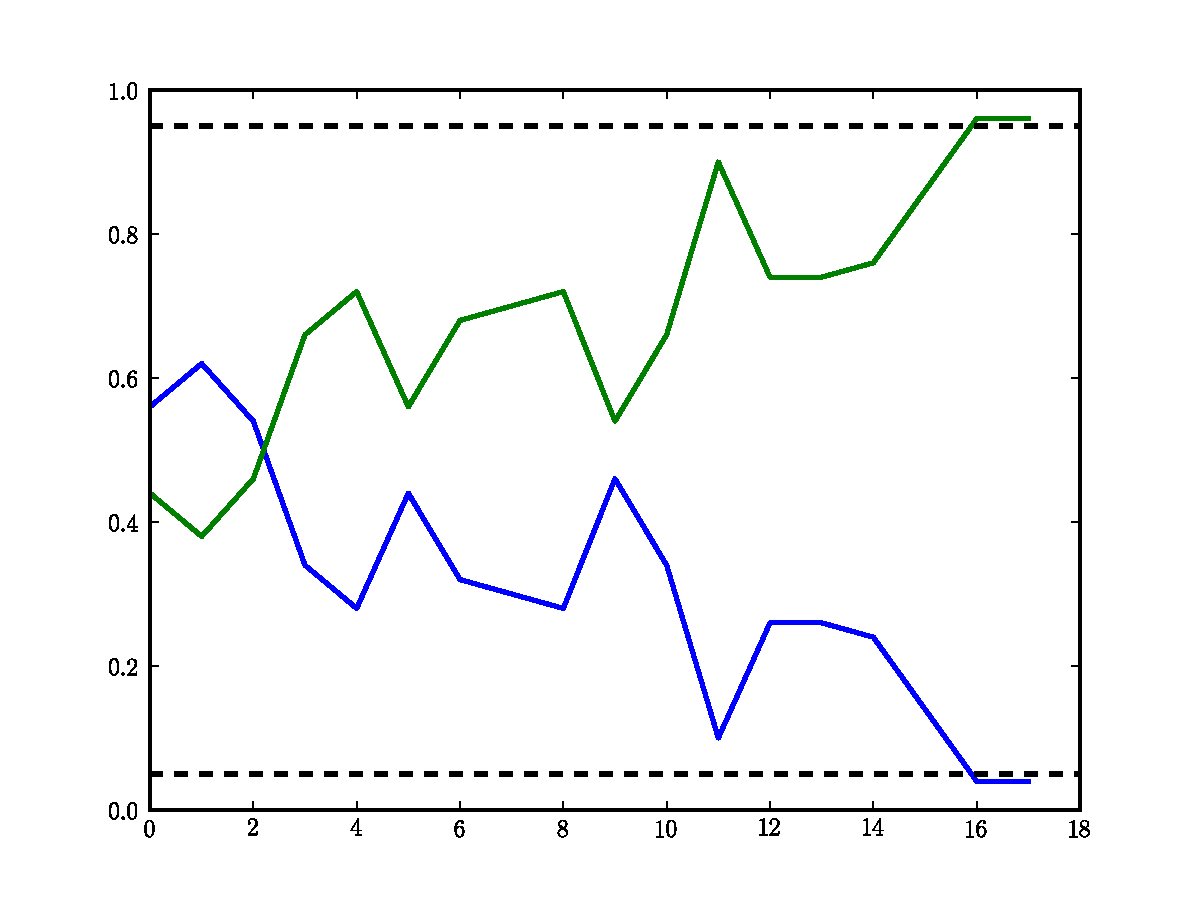
\includegraphics[width=\textwidth]{weights1.pdf}
\caption{Optimal arm probabilities in the two arm case}
\label{fig:weights1}
\end{subfigure}

\begin{subfigure}[t]{.49\textwidth}
\centering
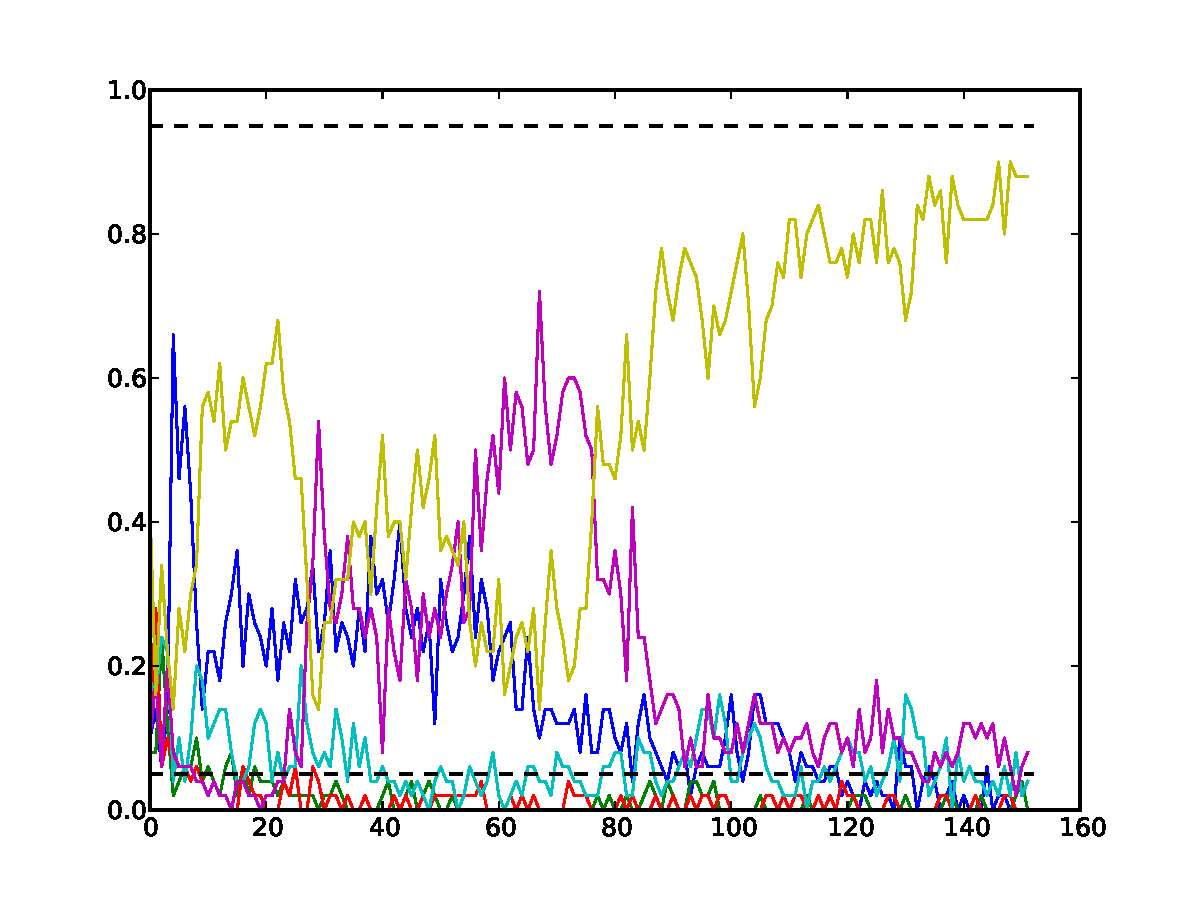
\includegraphics[width=\textwidth]{weights2.pdf}
\caption{Optimal arm probabilities in the six arm case}
\label{fig:weights2}
\end{subfigure}
\end{figure}

% \begin{figure}[h]
% \centering
% 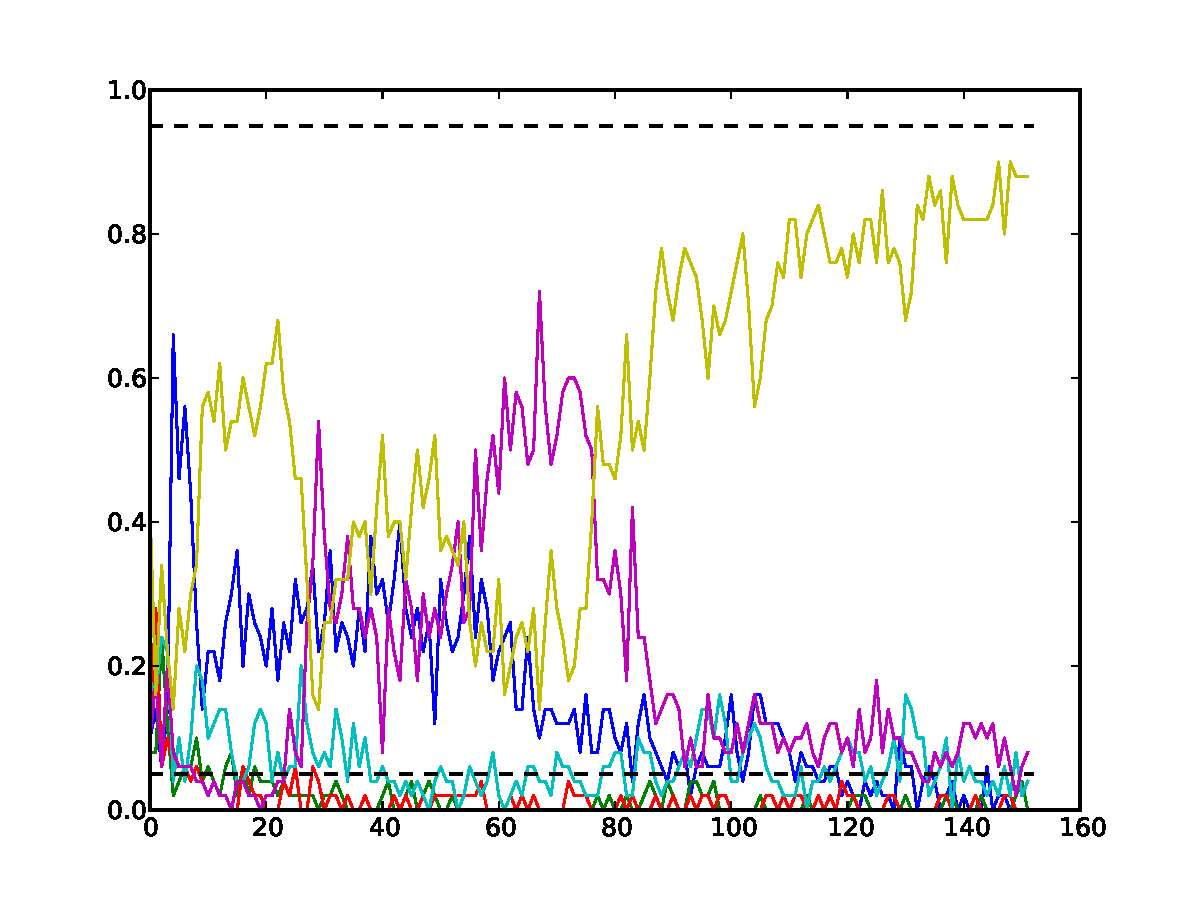
\includegraphics[width=\textwidth]{weights2.pdf}
% \caption{Optimal arm probabilities in the six arm case}
% \label{fig:weights2}
% \end{figure}


\section*{Comparison with Classical Tests}
A more classical approach to this problem would be to split traffic between each 
variation for a predetermined amount of time, which should give enough data to 
determine the best arm with some level of confidence.  
Using the bandit approach described here has significant advantages over a classical test.  
There are two main reasons why the bandit approach is more efficient.

The first reason is that the bandit method generally converges more quickly.  
A standard test would require splitting the web page views between the different 
variations over a long period of time.  According to Google's explanation in the 
website mentioned at the beginning of this lab, the two arm case would take 223 days 
and the 6 arm case would take 919 days.  The results from the simulations you performed
should show that on average the bandit method finishes much faster.  
There are other ways we could choose our stopping criteria that may result in even shorter experiment times.
In general, we can always adjust the tolerance of our stopping criteria to shorten experiment time or increase accuracy.

The second reason the bandit approach is more efficient is that, as we gain more information,
we allocate more visits to the variation that we believe has a better CvR.
In the classical method we would split the visits evenly until the end of the experiment.
This way we gain many more conversions during testing than we would using classical tests.
